\chapter{Data Understanding}

\section{Initial Data Collection Report}

\subsection{Data Requirements Planning}
The business objective is the development of a solution for the automatic aggregation of documents based on their topics. To achieve this goal, a sufficient number of documents are required. Also, the documents must contain enough text to be assigned a topic. After clustering the value of each expense in a cluster have to be summed, to gain the desired insight of spendings in one category. So the value an expense amounts to has to be included in the data.

\subsection{Selection Criteria}
An initial look a the data has shown that each invoice item can easily contain more than 100 pieces of information, which can be considered as attributed in the dataset. The part of the data that is of interest for the research is the description and payment data. Other data needs to be retained for a coherent and informative presentation of the results, such as location information and information on seller and buyer.

\subsection{Insertion of Data}

The insertion of data is concerned with the theoretical utilization of the data and problems arising during this process. The encoding and grouping of free text items is referenced as one concern in the \ac{CRISP-DM} user guide \cite{CRISPDM2000}. In this research the focus is on free text items, therefore this step will be discussed in detail in the following chapter. 
Other concerns are missing attributes. The dataset has already undergone a surface-level evaluation, which concludes that all relevant attributes are contained.

\section{Data Description Report}
The data is available as a local folder of size 5.12 GB, it contains 152,592 \ac{JSON} files. Each \ac{JSON} represents one invoice document. 
How many features per invoice?
What are the features?
Are there correlations between the attributes?
basic statistics for each significant attribtue

\begin{figure}[ht]
	\centering
	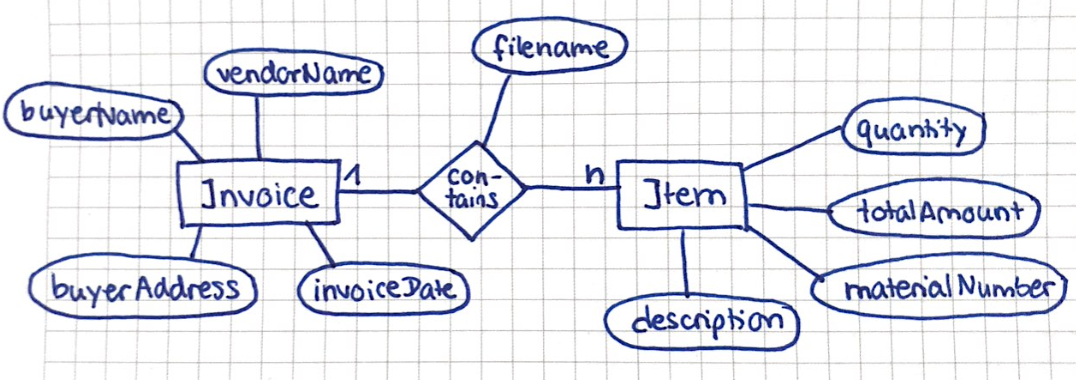
\includegraphics[height=5cm]{Bilder/practical/entity_relationship.png}
	\caption{Entity Relationship Diagram for Invoice Documents}
	\label{fig:er}
\end{figure}

\section{Data Exploration Report}
In which language are they written?
Form a hypothesis?

\section{Data Quality Report}
DOes the data contain errors?
Are there missing values?
are all values plausible?
plot some stuff here
check number of fields in each record (?) maybe optional
